\documentclass{article}
%packages
% \usepackage{tocloft}
\usepackage{polski}
\usepackage{amsmath}
\usepackage[utf8]{inputenc}
\usepackage{graphicx}
\usepackage{indentfirst}
\usepackage{float}
\usepackage[font=small,labelfont=bf]{caption}
\usepackage[polish]{babel}
\usepackage{hyperref}
\hypersetup{
    colorlinks,
    citecolor=black,
    filecolor=black,
    linkcolor=black,
    urlcolor=black
}
% Variables
\newcommand{\HRule}{\rule{\linewidth}{0.5mm}}
\newcommand{\Prowadzacy}{dr hab. inż. Robert \textsc{Nowicki} prof. PCz}
\newcommand{\Ja}{Piotr \textsc{Filek}\\101311\\I grupa}
\newcommand{\DataLaboratorium}{8 października 2013}
\newcommand{\Uczelnia}{ \textsc{\LARGE Politechnika Częstochowska}\\[1.5cm]}
\newcommand{\Przedmiot}{ \textsc{\Large Podstawy Sieci Komputerowych}\\[1.5cm]}
\newcommand{\TytulLaboratirum}{Laboratorium 1\\Sieci współdzielone}
\frenchspacing




\setlength{\intextsep}{20pt plus 1.0pt minus 2.0pt}

%Equations list
% \newcommand{\listequationsname}{List of Equations}
% \newlistof{myequations}{equ}{\listequationsname}
% \newcommand{\myequations}[1]{%
% \addcontentsline{equ}{myequations}{\protect\numberline{\theequation}#1}\par}

\begin{document}
\begin{titlepage}
\begin{center}
\Uczelnia
% \textsc{\LARGE Politechnika Częstochowska}\\[1.5cm]
\Przedmiot% \textsc{\Large Final year project}\\[0.5cm]
\HRule\\[0.4cm]
{ \huge \bfseries \TytulLaboratirum \\[0.4cm] }
% { \huge \bfseries Large brewing techniques \\[0.4cm]}
\HRule\\[1.5cm]

% Author and supervisor
\begin{minipage}[t]{0.4\textwidth}
\begin{flushleft}\large
\emph{Autor:}\\
\Ja
\end{flushleft}
\end{minipage}
\begin{minipage}[t]{0.5\textwidth}
\begin{flushright} \large
\emph{Prowadzący:} \\
\Prowadzacy
\end{flushright}
\end{minipage}

\vfill

% Bottom of the page
{\large \DataLaboratorium}

\end{center}
\end{titlepage}
% \begin{tableofcontents}
%   \listoffigures
% \end{tableofcontents}
\newpage
\section{Cel laboratorium}
Celem laboratorium była obserwacja działania współdzielonej sieci \linebreak Ethernet w funkcji stacji za pomocą symulatora takiej sieci oraz badanie niektórych parametrów sieci.
\section{Wyniki}
Poniższe symulacje zostały przeprowadzone dla punktu pomiarowego z \textbf{32 stacjami}, o \textbf{rozmiarze pakietu 1000} z opcją \textbf{ethernet\_advanced} w \textbf{Select Technologies}, oraz parametrze \textbf{Center Node Model} ustawionym na wartość \textbf{ethernet64\_hub\_adv}.
\begin{figure}[H]
  \centering
  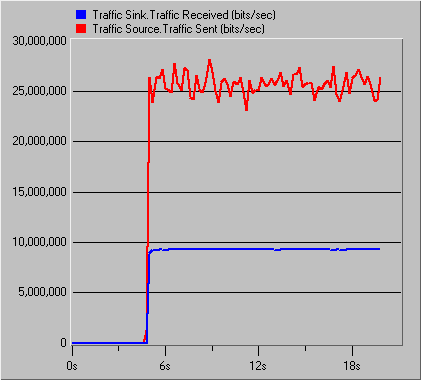
\includegraphics[width=0.65\textwidth]{screens/samo/001_sentrec.png}
 \caption{Wykres przedstawiający liczbę bitów wysłanych oraz liczbę bitów odebranych przez stacje przy \textbf{Interarrival time} ustawionym na 0.01. }
 \label{fig:sentrec001}
\end{figure}
 
\begin{figure}[H]
  \centering
  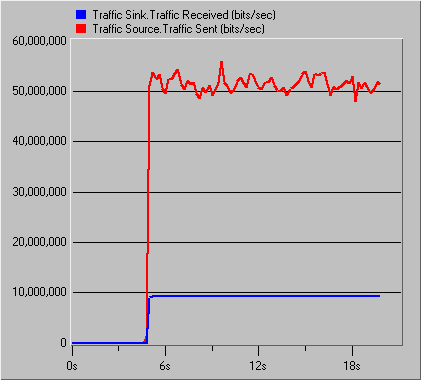
\includegraphics[width=0.65\textwidth]{screens/samo/0005_sentrec.png}
 \caption{Wykres przedstawiający liczbę bitów wysłanych oraz liczbę bitów odebranych przez stacje przy \textbf{Interarrival time} ustawionym na 0.005. }
 \label{fig:sentrec005}
\end{figure}

\begin{figure}[H]
  \centering
  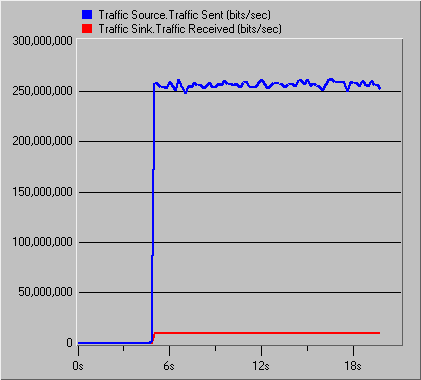
\includegraphics[width=0.65\textwidth]{screens/samo/0001_sentrec.png}
 \caption{Wykres przedstawiający liczbę bitów wysłanych oraz liczbę bitów odebranych przez stacje przy \textbf{Interarrival time} ustawionym na 0.001. }
 \label{fig:sentrec0001}
\end{figure}



\begin{figure}[H]
  \centering
  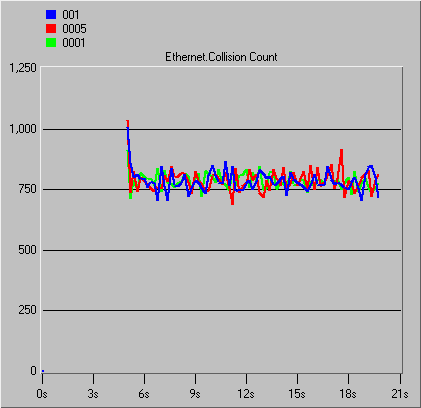
\includegraphics[width=0.65\textwidth]{screens/samo/koncentrator_collisioncount.png}
  \caption{Wykres przedstawiający ilość kolizji w koncentratorze.}
  \label{fig:collisioncount}
\end{figure}

\begin{figure}[H]
  \centering
  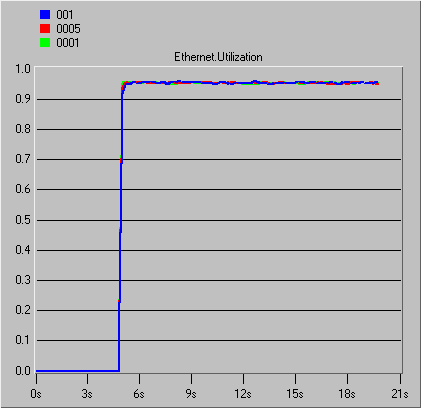
\includegraphics[width=0.65\textwidth]{screens/samo/koncentrator_utilization.png}
  \caption{Wykres przedstawiający wykorzystanie koncentratora.}
  \label{fig:utilization}
\end{figure}


\begin{figure}[H]
  \centering
  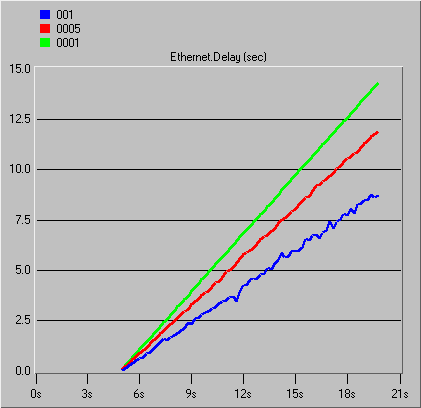
\includegraphics[width=0.65\textwidth]{screens/samo/delay.png}
  \caption{Wykres przedstawiający opóźnienia.}
  \label{fig:delay}
\end{figure}

\section{Wnioski}
Liczba pakietów wysłanych (Rysunek \ref{fig:sentrec001}, \ref{fig:sentrec005}, \ref{fig:sentrec0001}) zwiększa się wraz ze zwiększeniem częstotliwości ich wysyłania. Im większe obciążenie sieci, tym bardziej zwiększa się różnica pomiędzy pakietami wysłanymi i odebranymi - jest to spowodowane sposobem działania koncentratora, który nie może określić źródła ani miejsca docelowego odbieranych informacji, wysyła je do wszystkich połączonych z nim komputerów. Sygnał z portu wejściowego na \emph{wszystkie} porty wyjściowe bit po bicie.

Ilość kolizji (Rysunek \ref{fig:utilization}) oraz wykorzystanie koncentratora (Rysunek \ref{fig:collisioncount}) są podobne dla wszystkich scenariuszy, jednakże opóźnienia (Rysunek \ref{fig:delay}) wzrastają wraz ze zwiększeniem ilości wysyłanych pakietów. Jest to spowodowane tym, że koncentrator może wysyłać i odbierać informacje, jednak nie jednocześnie.

\end{document}